%%%%%%%%%%%%%%%%%%%%%%%%%%%%%%%%%%%%%%%%%%%%%%%%%%%%%%%%%%%%%%%%
\section{ハミルトン閉路問題および関連問題のASP符号化}\label{chap:proposal}
%%%%%%%%%%%%%%%%%%%%%%%%%%%%%%%%%%%%%%%%%%%%%%%%%%%%%%%%%%%%%%%% 

%%%%
\begin{figure*}[h]
  \centering
  \thicklines
  \setlength{\unitlength}{1.2pt}
  \small\footnotesize\scriptsize\tiny
  \begin{picture}(280,57)(4,-10)
    \put(  0, 20){\dashbox(50,24){\shortstack{HCP問題\\インスタンス}}}
    \put( 60, 20){\framebox(50,24){変換器}}
    \put(120, 20){\dashbox(50,24){\shortstack{ASPファクト}}}
    \put(120,-10){\dashbox(50,24){\shortstack{ASP符号化\\(論理プログラム)}}}
    \put(180, 20){\framebox(50,24){ASPシステム}}
    \put(240, 20){\dashbox(50,24){\shortstack{HCP問題\\の解}}}
    \put( 50, 32){\vector(1,0){10}}
    \put(110, 32){\vector(1,0){10}}
    \put(170, 32){\vector(1,0){10}}
    \put(230, 32){\vector(1,0){10}}
    \put(170, +2){\line(1,0){4}}
    \put(174, +2){\line(0,1){30}}
  \end{picture}  
\caption{ASP を用いたハミルトン閉路問題(HCP)の解法}
\label{fig:arch}
\end{figure*}
%%%%

%\begin{figure}[tbp]
\tikz{
  %1ノード目
  \path[draw=black, fill=blue!20, rounded corners=5pt]%線の設定
  node[at={(0.75,0.75)}] {問題}%文字を入れる
  (0,0) --(1.5,0) --(1.5,1.5) --(0,1.5) --cycle;%外周
  %2ノード目
  \path[draw=black, fill=blue!20, rounded corners=5pt, shift={(3,0)}]
  node[at={(0.75,0.75)}] {
    \begin{tabular}{c}
      ASP\\
      ファクト
    \end{tabular}
  }
  (0,0) --(1.5,0) --(1.5,1.5) --(0,1.5) --cycle;
  %3ノード目文字が複数行
  \path[draw=black, fill=green!20, rounded corners=5pt, shift={(6,0)}]
  node[at={(0.75,0.75)}] {
    \begin{tabular}{c}
      ASP\\
      システム
    \end{tabular}
  }
  (0,0) --(1.5,0) --(1.5,1.5) --(0,1.5) --cycle;
  %4ノード目文字が複数行
  \path[draw=black, fill=blue!20, rounded corners=5pt, shift={(9,0)}]
  node[at={(0.75,0.75)}] {解集合}
  (0,0) --(1.5,0) --(1.5,1.5) --(0,1.5) --cycle;
  %5ノード目文字が複数行
  \path[draw=black, fill=red!20, rounded corners=5pt, shift={(3,-3)}]
  node[at={(0.75,0.75)}] {
    \begin{tabular}{c}
      ASP\\
      符号化
    \end{tabular}
  }
  (0,0) --(1.5,0) --(1.5,1.5) --(0,1.5) --cycle;
  \draw[arrows=->] (1.5,0.75) --(3.0,0.75);
  \draw[arrows=->,shift={(3,0)}] (1.5,0.75) --(3.0,0.75);
  \draw[arrows=->,shift={(6,0)}] (1.5,0.75) --(3.0,0.75);
  \draw[arrows=->] (4.5,-2.25) --(6.0,0.5);
}
\caption{ASPを用いた解法}
\label{aspmethod}
\end{figure}


ASP を用いたハミルトン閉路問題および関連問題の解法について述べる.
図~\ref{fig:arch}に,解法の流れを示す.
与えられたハミルトン閉路問題は ASP ファクトに変換され,
ハミルトン閉路問題を解く ASP 符号化と結合され,
ASP システムによって解が計算される.
本論文では,ASP システムとして{\clingo}を用いる.

%%%%%%%%%%%%%%%%%%%%%%%%%%%%%%%%%%%%%%%%%%%%%%%%%%%%%%%%%%%%%%%%%%%%%%%
\subsection{ASPファクト形式}
%%%%%%%%%%%%%%%%%%%%%%%%%%%%%%%%%%%%%%%%%%%%%%%%%%%%%%%%%%%%%%%%%%%%%%%

%%%%%%%%%%%%%%%%%%%%%%%%%%%%%%
\begin{figure}[tb]
\begin{center}
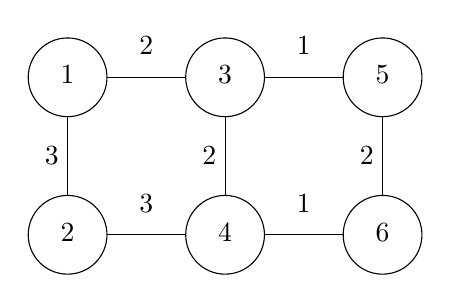
\begin{tikzpicture}
  %ノード1  
  \draw(4,2) circle (0.5)
  node[at={(4.0,2.0)}] {
    \begin{tabular}{c}
      1
    \end{tabular}
  };
  %ノード2  
  \draw(4,0) circle (0.5)
  node[at={(4.0,0.0)}] {
    \begin{tabular}{c}
      2
    \end{tabular}
  };
  %ノード3  
  \draw(6,2) circle (0.5)
  node[at={(6.0,2.0)}] {
    \begin{tabular}{c}
      3
    \end{tabular}
  };
  %ノード4  
  \draw(6,0) circle (0.5)
  node[at={(6.0,0.0)}] {
    \begin{tabular}{c}
      4
    \end{tabular}
  };
  %ノード5  
  \draw(8,2) circle (0.5)
  node[at={(8.0,2.0)}] {
    \begin{tabular}{c}
      5
    \end{tabular}
  };
  %ノード6  
  \draw(8,0) circle (0.5)
  node[at={(8.0,0.0)}] {
    \begin{tabular}{c}
      6
    \end{tabular}
  };
  \draw(4,0.5) --(4,1.5)
  node[at={(3.8,1.0)}] {3};
  \draw(6,0.5) --(6,1.5)
  node[at={(5.8,1.0)}] {2};
  \draw(8,0.5) --(8,1.5)
  node[at={(7.8,1.0)}] {2};
  \draw(4.5,0) --(5.5,0)
  node[at={(5.0,0.4)}] {3};
  \draw(4.5,2) --(5.5,2)
  node[at={(5.0,2.4)}] {2};
  \draw(6.5,0) --(7.5,0)
  node[at={(7.0,0.4)}] {1};
  \draw(6.5,2) --(7.5,2)
  node[at={(7.0,2.4)}] {1};
\end{tikzpicture}

\caption{入力となる重み付き無向グラフの例}
\label{graphexample}
\end{center}
\end{figure}
%%%%%%%%%%%%%%%%%%%%%%%%%%%%%%

%%%%%%%%%%%%%%%%%%%%%%%%%%%%%%
\lstinputlisting[float=t,caption={%
図~\ref{graphexample}のASPファクト表現},%
captionpos=b,frame=single,label=code:graph_example.lp,%
numbers=none,%
breaklines=true,%
columns=fullflexible,keepspaces=true,%
basicstyle=\ttfamily\scriptsize]{code/graph_example.lp}
%%%%%%%%%%%%%%%%%%%%%%%%%%%%%%


本節では,最短ハミルトン閉路問題の例にとって,
入力となる重み付き無向グラフ(図~\ref{graphexample})の
ASP ファクト形式について説明する.
%
このグラフは,頂点数が6,辺の数が7であり,辺に付けられた値は距離を表す.
コード~\ref{code:graph_example.lp}に,ASPファクト形式を示す.
%
アトム\code{node/1}は頂点,\code{edge/2}は辺,\code{cost/3}は距離を表す.
例えば,\code{cost(1,2,3)}は,辺\code{edge(1,2)}の距離が3であることを
表している.

%%%%%%%%%%%%%%%%%%%%%%%%%%%%%%%%%%%%%%%%%%%%%%%%%%%%%%%%%%%%%%%%%%%%%%%
\subsection{ハミルトン閉路問題の ASP 符号化}\label{hamiltonianasp}
%%%%%%%%%%%%%%%%%%%%%%%%%%%%%%%%%%%%%%%%%%%%%%%%%%%%%%%%%%%%%%%%%%%%%%%

ハミルトン閉路問題は,与えられたグラフの全頂点をちょうど一度ずつ通る閉
路(ハミルトン閉路)が存在するかどうかを判定する問題である.
$G=(V,E)$にハミルトン閉路が存在する必要十分条件は,
以下の2つの制約を満たす部分グラフ$G'=(V,E')$が存在することである.

\begin{itemize}
\item $G'$の各頂点の次数が2 (次数制約)
\item $G'$が連結である (連結制約)
\end{itemize}

本論文では,前者を\textbf{次数制約},後者を\textbf{連結制約}と呼ぶ.
ハミルトン路問題は,ハミルトン閉路問題から始点と終点が一致するという閉
路の条件を取り除いたものである.
ハミルトン路問題では,次数制約は以下のように変わる.

\begin{itemize}
\item 始点と終点の次数が1,他の頂点の次数が2
\end{itemize}

以下では,ハミルトン閉路問題に対する3つの ASP 符号化
\textsf{undirected},\textsf{directed},\textsf{acyclicity}
を提案する.

%%%%%%%%%%%%%%%%%%%%%%%%%%%%%%%%%%%%%%%%%%%%%%%%%%%%%%%%%%%%%%%%%%%%%%%
\subsubsection{\textsf{undirected}符号化}
%%%%%%%%%%%%%%%%%%%%%%%%%%%%%%%%%%%%%%%%%%%%%%%%%%%%%%%%%%%%%%%%%%%%%%%

%%%%%%%%%%%%%%%%%%%%%%%%%%%%%%
\lstinputlisting[float=t,caption={%
\textsf{undirected}符号化},%
captionpos=b,frame=single,label=code:hamilton1.lp,%
numbers=left,%
breaklines=true,%
columns=fullflexible,keepspaces=true,%
basicstyle=\ttfamily\footnotesize]{code/hamilton1.lp}
%%%%%%%%%%%%%%%%%%%%%%%%%%%%%%

\textsf{undirected}符号化は,ハミルトン閉路問題の次数制約と連結制約を,
ASP の一貫性制約で表した基本的な符号化である.
コード~\ref{code:hamilton1.lp}に,\textsf{undirected}符号化を示す.
この符号化は,ハミルトン閉路問題とハミルトン路問題の両方に対応している.
符号化中の\code{s}は始点の頂点番号,\code{t}は終点の頂点番号を表し,こ
れらは実行時に与えられる.
ここでは,ハミルトン閉路問題(\code{s}=\code{t})の場合について説明する.

\begin{itemize}
\item 1行目のルールは,各辺\code{edge(X,Y)}に対して,その辺がハミルト
  ン閉路に含まれるかどうかを意味するアトム\code{in(X,Y)}を選択子を用い
  て導入している.
\item 次数制約は3行目のルールで表される.
  このルールは,各頂点\code{node(X)}に対して,
  その次数が2に等しいことを個数制約を使って表している.
\item 連結制約は11行目のルールで表される.
ある頂点\code{X}が始点\code{s}から到達可能であることを意味する補助アト
ム\code{reached(X)}を導入する.
8行目のルールは,始点\code{s}が到達可能あることを表している.
9行目のルールは,各辺\code{X}--\code{Y}に対して,その辺がハミルトン閉
路に含まれ(\code{in(X,Y)}),かつ,頂点\code{X}が始点から到
達可能であれば(\code{reached(X)}),\code{Y}も到達可能であることを表している.
10行目は9行目と同様であるが,辺\code{Y}--\code{X}の場合を表している.
11行目のルールは,各頂点\code{node(X)}が始点から到達可能でなければな
らないことを一貫性制約を使って表している.
\end{itemize}

%%%%%%%%%%%%%%%%%%%%%%%%%%%%%%%%%%%%%%%%%%%%%%%%%%%%%%%%%%%%%%%%%%%%%%%
\subsubsection{\textsf{directed}符号化}
%%%%%%%%%%%%%%%%%%%%%%%%%%%%%%%%%%%%%%%%%%%%%%%%%%%%%%%%%%%%%%%%%%%%%%%

%%%%%%%%%%%%%%%%%%%%%%%%%%%%%%
\lstinputlisting[float=t,caption={%
\textsf{directed}符号化},%
captionpos=b,frame=single,label=code:hamilton2.lp,%
numbers=left,%
breaklines=true,%
columns=fullflexible,keepspaces=true,%
basicstyle=\ttfamily\footnotesize]{code/hamilton2.lp}
%%%%%%%%%%%%%%%%%%%%%%%%%%%%%%

\textsf{directed}符号化は,\textsf{undirected}符号化をベースに,
与えられた無向グラフの各辺$u-v$に対して,2つの弧$u\rightarrow v$と
$v\rightarrow u$を対応させることで有向グラフ化して解く符号化である.
コード~\ref{code:hamilton2.lp}に,\textsf{directed}符号化を示す.
前節と同様に,ハミルトン閉路問題(\code{s}=\code{t})の場合について説明する.

\begin{itemize}
\item 1行目では,無向グラフの有向グラフ化を行う.
  与えられた無向グラフの各辺\code{edge(X,Y)}に対して,
  新たに\code{edge(Y,X)}を導入した.
\item 2行目のルールは,各弧\code{edge(X,Y)}に対して,その弧がハミルト
  ン閉路に含まれるかどうかを意味するアトム\code{in(X,Y)}を選択子を用い
  て導入している.
\item 次数制約は4,5行目のルールで表される.
  4行目では,各頂点\code{node(X)}に対して,
  その出次数が1に等しいことを個数制約を使って表している.
  5行目では,入次数について4行目と同様の制約を表す.
\item 連結制約は15行目のルールで表される.
  ある頂点\code{X}が始点\code{s}から到達可能であることを意味する
  補助アトム\code{reached(X)}を導入する.
  13行目のルールは,始点\code{s}が到達可能あることを表している.
  14行目のルールは,各弧\code{X}--\code{Y}に対して,その弧がハミルトン閉路
  に含まれ(\code{in(X,Y)}),かつ,頂点\code{X}が始点から
  到達可能であれば(\code{reached(X)}),\code{Y}も到達可能であることを表している.
  15行目のルールは,各頂点\code{node(X)}が始点から到達可能でなければ
  ならないことを一貫性制約を使って表している.
\item 18行目のルールは,解についての対称性を除去する.
  与えられた無向グラフ上の各ハミルトン閉路に対して,
  それを変換した有向グラフ上のハミルトン閉路は対称な2つが存在する.
  これによる解の重複を防ぐために,18行目のルールは,各弧\code{s}--\code{X},
  \code{Y}--\code{s}がハミルトン閉路に含まれるならば(\code{in(s,X),in(Y,s)}),
  \code{X < Y}でなければならないことを,一貫性制約を用いて表している
\end{itemize}

%%%%%%%%%%%%%%%%%%%%%%%%%%%%%%%%%%%%%%%%%%%%%%%%%%%%%%%%%%%%%%%%%%%%%%%
\subsubsection{\textsf{acyclicity}符号化}
%%%%%%%%%%%%%%%%%%%%%%%%%%%%%%%%%%%%%%%%%%%%%%%%%%%%%%%%%%%%%%%%%%%%%%%

%%%%%%%%%%%%%%%%%%%%%%%%%%%%%%
\lstinputlisting[float=t,caption={%
\textsf{acyclicity}符号化},%
captionpos=b,frame=single,label=code:hamilton3.lp,%
numbers=left,%
breaklines=true,%
columns=fullflexible,keepspaces=true,%
basicstyle=\ttfamily\footnotesize]{code/hamilton3.lp}
%%%%%%%%%%%%%%%%%%%%%%%%%%%%%%

\textsf{acyclicity}符号化は,\textsf{directed}符号化をベースに,
連結制約を部分閉路を禁止する制約に置き換え,それを ASP の$\#edge$宣言
で表現した符号化である.
コード~\ref{code:hamilton3.lp}に,\textsf{acyclicity}符号化を示す.
\textsf{directed}符号化との違いは,13--14行目だけである.
前節と同様に,ハミルトン閉路問題(\code{s}=\code{t})の場合について説明する.

\begin{itemize}
% \item 1行目では,無向グラフの有向グラフ化を行う.
%   与えられた無向グラフの各辺\code{edge(X,Y)}に対して,
%   2つの弧\code{edge(X,Y)},\code{edge(Y,X)}を導入した.
% \item 2行目のルールは,各弧\code{edge(X,Y)}に対して,その弧がハミルト
%   ン閉路に含まれるかどうかを意味するアトム\code{in(X,Y)}を選択子を用い
%   て導入している.
% \item 次数制約は4,5行目のルールで表される.
%   4行目では,各頂点\code{node(X)}に対して,
%   その出次数が1に等しいことを個数制約を使って表している.
%   5行目では,入次数について4行目と同様の制約を表す.
\item  14行目のルールは,\code{in(X,Y)}を満たす弧集合をもつグラフが閉
  路を含まないことを,$\#edge$宣言を用いて表している.ただし,
  \code{X}と\code{Y}は始点ではない.
%\item 17行目のルールは,解についての対称性を除去する.
%   与えられた無向グラフ上の各ハミルトン閉路に対して,
%   それを変換した有向グラフ上のハミルトン閉路は対称な2つが存在する.
%   これによる解の重複を防ぐために,17行目のルールは,各弧\code{s}--\code{X},
%   \code{Y}--\code{s}がハミルトン閉路に含まれるならば(\code{in(s,X),in(Y,s)}),
%   \code{X < Y}でなければならないことを,一貫性制約を用いて表している
\end{itemize}

%%%%%%%%%%%%%%%%%%%%%%%%%%%%%%%%%%%%%%%%%%%%%%%%%%%%%%%%%%%%%%%%%%%%%%% 
\subsection{最短ハミルトン閉路問題のASP符号化}\label{minexpl}
%%%%%%%%%%%%%%%%%%%%%%%%%%%%%%%%%%%%%%%%%%%%%%%%%%%%%%%%%%%%%%%%%%%%%%% 

%%%%%%%%%%%%%%%%%%%%%%%%%%%%%%
\lstinputlisting[float=ht,caption={%
ハミルトン閉路における距離の総和の最小化},%
captionpos=b,frame=single,label=code:obj_minimize.lp,%
numbers=none,%
breaklines=true,%
columns=fullflexible,keepspaces=true,%
basicstyle=\ttfamily\footnotesize]{code/obj_minimize.lp}
%%%%%%%%%%%%%%%%%%%%%%%%%%%%%%

%%%%%%%%%%%%%%%%%%%%%%%%%%%%%%
\lstinputlisting[float=ht,caption={%
\textsf{directed}符号化と\textsf{acyclicity}符号化のための補助ルール},%
captionpos=b,frame=single,label=code:cost_both.lp,%
numbers=none,%
breaklines=true,%
columns=fullflexible,keepspaces=true,%
basicstyle=\ttfamily\footnotesize]{code/cost_both.lp}
%%%%%%%%%%%%%%%%%%%%%%%%%%%%%%

最短ハミルトン閉路問題のASP符号化は,これまで説明した符号化に,
目的関数を追加することで実現できる.
最短ハミルトン閉路問題の目的関数は,ハミルトン閉路を構成する各辺の距離
の総和の最小化である.
コード\ref{code:obj_minimize.lp}に目的関数を示す.
このルールは,\code{#minimize}宣言を使って,
ハミルトン閉路に含まれる各辺\code{X}--\code{Y}の距離\code{C}
の総和を最小化している.

\textsf{directed}と\textsf{acyclicity}符号化については,
与えられた無向グラフの各辺
\code{X}--\code{Y}に対して,2つの弧
\code{X}$\rightarrow$\code{Y}と
\code{Y}$\rightarrow$\code{X}を対応させることで有向グラフ化している.
そのため,この2つの符号化には,
コード\ref{code:obj_minimize.lp}に加えて,
コード\ref{code:cost_both.lp}を追加する必要がある.
コード\ref{code:cost_both.lp}のルールは,各辺\code{X}--\code{Y}の距離
を表す\code{cost(X,Y,C)}について,\code{cost(Y,X,C)}を新たに導入している.

%%%%%%%%%%%%%%%%%%%%%%%%%%%%%%%%%%%%%%%%%%%%%%%%%%%%%%%%%%%%%%%%%%%%%%% 
\subsection{コスト制約付きハミルトン閉路問題のASP符号化}
%%%%%%%%%%%%%%%%%%%%%%%%%%%%%%%%%%%%%%%%%%%%%%%%%%%%%%%%%%%%%%%%%%%%%%% 

%%%%%%%%%%%%%%%%%%%%%%%%%%%%%%
\lstinputlisting[float=ht,caption={%
コスト制約},%
captionpos=b,frame=single,label=code:cost_constraint.lp,%
numbers=none,%
breaklines=true,%
columns=fullflexible,keepspaces=true,%
basicstyle=\ttfamily\footnotesize]{code/cost_constraint.lp}
%%%%%%%%%%%%%%%%%%%%%%%%%%%%%%

コスト制約付きハミルトン閉路問題は,
ハミルトン閉路問題に,距離の総和が所与の閾値以下 (または以上) であるこ
とを制約条件として付加した問題である.
コード\ref{code:cost_constraint.lp}に,その制約条件を示す.
ルール中の\code{c}は閾値を表し,これは実行時に与えられる.
このルールは,各辺\code{edge(X,Y)}に対して,その辺がハミルトン閉路に
含まれ(\code{in(X,Y)}),その距離が\code{C}である時に(\code{cost(X,Y,C)}),
\code{C}の総和が\code{c}以下でなければならないことを,
一貫性制約と重み付き個数制約を用いて表している.
また,\ref{minexpl}節と同様に,
\textsf{directed}と\textsf{acyclicity}符号化については,
アトム\code{cost/3}についても有向グラフ化に
対応させるためにコード\ref{code:cost_both.lp}を追加した.
%%%%%%%%%%%%%%%%%%%%%%%%%%%%%%%%%%%%%%%%%%%%%%%%%%%%%%%%%%%%%%%%%%%%%%%

%%% Local Variables:
%%% mode: latex
%%% TeX-master: "paper"
%%% End:
